\renewcommand{\theequation}{\theenumi}
\renewcommand{\thefigure}{\theenumi}
\renewcommand{\thetable}{\theenumi}
\begin{enumerate}[label=\thesection.\arabic*.,ref=\thesection.\theenumi]
\numberwithin{equation}{enumi}
\numberwithin{figure}{enumi}
\numberwithin{table}{enumi}



\item Let $Y_1$ denote the first order statistic in a random sample of size $n$ from a distribution that has the pdf 
\begin{align}
    f(x) = 
    \begin{cases}
    e^{-(x-\theta)}&\text{ when } \theta<x<\infty\\
    0 &\text{  otherwise} 
    \end{cases}
\end{align}
Obtain the distribution of $Z_n = n(Y_1 - \theta)$.
%
\\
\solution
From the given information
\begin{align}
    Y_1 = \min\{X_1, X_2, ... X_n\}
\end{align}
%
and
\begin{align}
    F_{Z_n}(z) &= \pr{n(Y_1-\theta)\leq z}\\
    &= \pr{Y_1\leq \frac{z}{n} +\theta}\\
    &= 1-\pr{Y_1\ > \frac{z}{n} +\theta}\label{stats/1/eq_2}
\end{align}
%
Let
\begin{align}
    \brak{\dfrac{z}{n}+\theta} = z^{\prime}
\end{align}
%
Then
\begin{align}
    F_{Z_n}\brak{z}    &= 1-\prod_{i=1}^{n}\pr{X_i>z^{\prime}}\\
    &= 1-\brak{1-F(z^{\prime})}^n\\
    \implies F_{Z_n}(z) &= 1-\brak{1-F\brak{\frac{z}{n}+\theta}}^n\label{stats/1/eq_3}
\end{align}
%
where
%
\begin{align}
  F(x) &=\displaystyle\int\limits_{-\infty}^{x} f(t) \,dt\\
&=
    \begin{cases}
    1-e^{-(x-\theta)} &\text{when }\theta<x<\infty\\
    0 &\text{otherwise}
    \end{cases}
    \label{stats/1/eq_1}
\end{align}
%
Substituting from     \eqref{stats/1/eq_1} in \eqref{stats/1/eq_3},
\begin{align}
    F_{Z_n}(z) &=
    \begin{cases}
    1-e^{-n\brak{\frac{z}{n}+\theta-\theta}}&  \theta<\frac{z}{n}+\theta<\infty\\
    0&\text{otherwise}
    \end{cases}\\
    &= \begin{cases}
    1-e^{-z}&\text{when } 0<z<\infty\\
    0 &\text{otherwise}\label{stats/1/cdf}
    \end{cases}
\end{align}
and 
\begin{align}
    f_{Z_n}(z) &= \frac{d}{dz}F_{Z_n}(z)\\
    &=\begin{cases}
    e^{-z}& 0<z<\infty\\
    0&\text{otherwise}
    \end{cases}\label{stats/1/pdf}
\end{align}
The plots for the cdf in \eqref{stats/1/cdf} and the pdf in \eqref{stats/1/pdf} are shown in Fig. \ref{stats/1/fig_cdf} and Fig. \ref{stats/1/fig_pdf} respectively:
\begin{figure}[!ht]
    \centering
    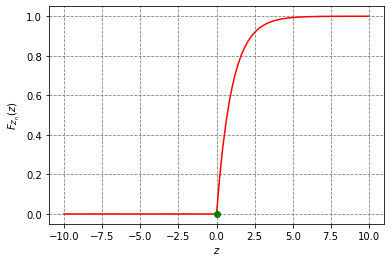
\includegraphics[width=\columnwidth]{stats/solutions/1/figures/cdf.png}
    \caption{cdf of $Z_n$}
    \label{stats/1/fig_cdf}
\end{figure}
\begin{figure}[!ht]
    \centering
    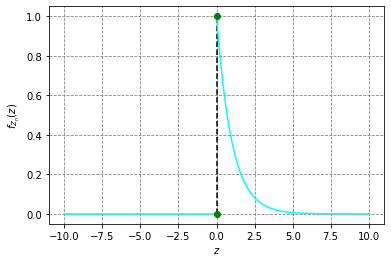
\includegraphics[width=\columnwidth]{stats/solutions/1/figures/pdf.png}
    \caption{pdf of $Z_n$}
    \label{stats/1/fig_pdf}
\end{figure}





\end{enumerate}